\documentclass{article}
\usepackage{eason}

\usepackage{pdfpages}

\usepackage[a4paper, margin=1in]{geometry}

\usepackage{lipsum}
\usepackage{multicol}

\newcommand{\DATE}{dummyDate}
\newcommand{\COMMITSHA}{dummySHA}

\title{TMUA Lecture 6 -- Logic and Proof}
\author{Eason Shao}
\date{v.\DATE.\COMMITSHA}

\begin{document}
\maketitle

\tableofcontents

\section{Logic of Arguments}

\subsection{Statements, True and False}

A (mathematical) \textbf{statement} is a sentence which is definitely true of definitely false. \textit{Law of Excluded Middle} states that a statement can only be either true or false, but not both. (This serves as the foundation to link Proof by Contradiction and by Contraposition.)

Statements often take the form of ``if \dots, then \dots.''

\begin{example}
    Determine whether the following sentences are statements.
    \begin{itemize}
        \item The equation \(x^3 + y^2 = 88\) has no integer solutions.
        \item What is your name?
        \item The number \(2147483647\) is a prime.
        \item If \(x^2 = 9\), then \(x = 3\).
        \item It will rain tomorrow.
        \item \(x + 2 = 5\).
    \end{itemize}
\end{example}

\begin{problem}[Barber's Problem, Russell's Paradox]
    Is the following sentence a statement: the only barber in a town shaves each and every man who does not shave himself.
\end{problem}

The \textbf{truth value} of a statement is, as the name suggests, whether the statement is true or false.

Two statements are \textbf{logically equivalent} if they have the same truth value under any circumstances.

\begin{example}[TMUA 2016 P2 Q4]
    Five sealed urns, labelled \(P\), \(Q\), \(R\), \(S\), and \(T\), each contain the \textbf{same} (non-zero) number of balls. The following statements are attached to the urns.

    \begin{itemize}
        \item \textbf{Urn \(P\).} This urn contains one or four balls.
        \item \textbf{Urn \(Q\).} This urn contains two or four balls.
        \item \textbf{Urn \(R\).} This urn contains more than two balls and fewer than five balls.
        \item \textbf{Urn \(S\).} This urn contains one or two balls.
        \item \textbf{Urn \(T\).} This urn contains fewer than three balls.
    \end{itemize}

    Exactly one of the urns has a true statement attached to it. Which urn is it?
\end{example}

\subsection{And, Or, Not}

If we have two statements \(A\) and \(B\), we may combine them using certain logical symbols:
\begin{itemize}
    \item \textbf{and}, denoted \(A \land B\), has truth value true exactly when both \(A\) and \(B\) are true;
    \item \textbf{or}, denoted \(A \lor B\), has truth value true exactly when at least one of \(A\) and \(B\) are true (inclusive or, i.e. if \(A \land B\) is true, then \(A \lor B\) is true).
\end{itemize}

For a single statement \(A\), the \textbf{not} operator, denoted \(\lnot A\), has truth value true exactly when \(A\) is false.

And and Or are both commutative and associative, and distributes over each other.

Suppose \(S\) and \(T\) are situations (e.g. values of \(x\)) that make \(A\) and \(B\) true, respectively. Then the situations that make:
\begin{itemize}
    \item \(A \land B\) true, is \(S \cap T\)
    \item \(A \lor B\) true, is \(S \cup T\)
    \item \(\lnot A\) true, is \(S\compl\) (the complement of the set \(S\))
\end{itemize}

We have the following rules:
\begin{itemize}
    \item \textbf{Commutativity.} \(A \land B = B \land A\); \(A \lor B = B \lor A\);
    \item \textbf{Associativity.} \(\pqty{A \land B} \land C = A \land \pqty{B \land C}\); \(\pqty{A \lor B} \lor C = A \lor \pqty{B \lor C}\)
    \item \textbf{Distributivity.} \(\pqty{A \land B} \lor C = \pqty{A \lor C} \land \pqty{B \lor C}\); \(\pqty{A \lor B} \land C = \pqty{A \land C} \lor \pqty{B \land C}\);
    \item \textbf{Double negation.} \(\lnot \pqty{\lnot A} = A\);
    \item \textbf{De Morgan's Laws.} \(\lnot \pqty{A \land B} = \pqty{\lnot A} \lor \pqty{\lnot B}\); \(\lnot \pqty{A \lor B} = \pqty{\lnot A} \land \pqty{\lnot B}\)
\end{itemize}

\begin{example}
    Let \(x \in \RR\). Let \(A\) be the statement \(-3 < x < 3\), and \(B\) be the statement \(-2 < x < 4\). Find the statements \(A \land B\), \(A \lor B\), and \(\lnot A\).
\end{example}

\subsection{Implies, Sufficient and Necessary}

For two statements \(A\) and \(B\), the \(7\) statements
\begin{multicols}{2}
    \begin{itemize}
        \item \textbf{if \(A\) then \(B\)},
        \item \textbf{\(B\) if \(A\)},
        \item \textbf{\(A\) only if \(B\)},
        \item \textbf{\(A\) implies \(B\)},
        \item \textbf{\(B\) is implied by \(A\)},
        \item \textbf{\(A\) is a sufficient condition for \(B\)},
        \item \textbf{\(B\) is a necessary condition for \(A\)}
    \end{itemize}
\end{multicols}
are all equivalent, and denoted \(A \implies B\) or \(B \implies A\). The resulting statement is true, precisely when \textbf{all possible situations that make \(A\) true make \(B\) true}.

\begin{example}
    The following statements are all equivalent (and true):
    \begin{multicols}{2}
        \begin{itemize}
            \item if \(x = -3\) then \(x^2 = 9\),
            \item \(x^2 = 9\) if \(x = -3\),
            \item \(x = -3\) only if \(x^2 = 9\),
            \item \(x = -3\) implies \(x^2 = 9\),
            \item \(x^2 = 9\) is implied by \(x = -3\),
            \item \(x = -3\) is a sufficient condition for \(x^2 = 9\),
            \item \(x^2 = 9\) is a necessary condition for \(x = -3\)
        \end{itemize}
    \end{multicols}
\end{example}

The statements
\begin{itemize}
    \item \textbf{\(A\) if and only if \(B\)},
    \item \textbf{\(B\) if and only if \(A\)},
    \item \textbf{\(A\) is necessary and sufficient for \(B\)},
    \item \textbf{\(B\) is necessary and sufficient for \(A\)},
    \item \textbf{\(A\) and \(B\) are equivalent}
\end{itemize}
are all equivalent. This is denoted \(A \iff B\).

It is often useful to think about implication using set notation. Suppose \(S\) and \(T\) are situations (e.g. values of \(x\)) that make \(A\) and \(B\) true, respectively. Then \(A \implies B\) is true precisely when \(S \subseteq T\). (This is the so-called ``a smaller set implies a bigger set''.) \(A \iff B\) therefore corresponds to \(S = T\).

\begin{example}
    Consider the following six statements:
    \begin{multicols}{2}
        \begin{itemize}
            \item If it is Sunday, then the church bells ring.
            \item It is Sunday if the church bells ring.
            \item It is Sunday only if the church bells ring.
            \item If the church bells ring, then it is Sunday.
            \item The church bells ring if it is Sunday.
            \item The church bells ring only if it is Sunday.
        \end{itemize} 
    \end{multicols}

    Consider the following four observations:
    \begin{multicols}{2}
        \begin{itemize}
            \item It is Sunday.
            \item It is not Sunday.
            \item The church bells ring.
            \item The church bells do not ring.
        \end{itemize}
    \end{multicols}
    

    What cam we imply (if any) from each of the possible 24 pairings of the statement and the observation?
\end{example}

\begin{example}[TMUA 2016 P2 Q10]
    In this question \(x\) and \(y\) are non-zero real numbers. Which one of the following is \textbf{sufficient} to conclude that \(x < y\)?
    
    \begin{multicols}{3}
        \begin{enumerate}[label=\Alph*.]
            \item \(x^4 < y^4\)
            \item \(y^4 < x^4\)
            \item \(x\inverse < y\inverse\)
            \item \(y\inverse < x\inverse\)
            \item \(x^{\flatfrac{3}{5}} < y^{\flatfrac{3}{5}}\)
            \item \(y^{\flatfrac{3}{5}} < x^{\flatfrac{3}{5}}\)
        \end{enumerate}
    \end{multicols}
\end{example}

\begin{example}[TMUA 2017 P2 Q10]
    \(f\pqty{x}\) is a function defined for all real values of \(x\). Which one of the following is a \textbf{sufficient} condition for \(\int_1^3 f\pqty{x} \dd{x} = 0\)?

    \begin{multicols}{2}
        \begin{enumerate}[label=\Alph*.]
            \item \(f\pqty{2} = 0\)
            \item \(f\pqty{1} = f\pqty{3} = 0\)
            \item \(f\pqty{-x} = - f\pqty{x}\) for all \(x\)
            \item \(f\pqty{x + 2} = - f\pqty{2 - x}\) for all \(x\)
            \item \(f\pqty{x - 2} = - f\pqty{2 - x}\) for all \(x\)
        \end{enumerate}
    \end{multicols}
\end{example}

Negating implications are as follows:
\[
    \lnot \pqty{A \implies B} = A \land \pqty{\lnot B}
\]
since for \(A\) to not imply \(B\), we need to have \(A\) is true while \(B\) is not true.

\begin{problem}
    What is the difference between ``\(A \implies B\)'' and ``\(A\), therefore \(B\)''?
\end{problem}

\subsection{Converse, Inverse and Contrapositive}

For a statement of the form \(A \implies B\), its
\begin{itemize}
    \item \textbf{converse} is \(B \implies A\);
    \item \textbf{inverse} is \(\lnot A \implies \lnot B\);
    \item \textbf{contrapositive} is \(\lnot B \implies \lnot A\).
\end{itemize}

The TMUA does not require knowledge about the inverse.

\begin{example}
    For the statement \(x = -3 \implies x^2 = 9\):
    \begin{itemize}
        \item its converse is \(x^2 = 9 \implies x = -3\);
        \item its inverse is \(x \neq -3 \implies x^2 \neq 9\);
        \item its contrapositive is \(x^2 \neq 9 \implies x \neq -3\).
    \end{itemize}
\end{example}

A statement is \textbf{equivalent to its contrapositive}.

\begin{example}
    Let \(x \in \ZZ\). Prove the statement: if \(x^2\) is odd, then \(x\) is odd.
\end{example}

\subsection{Quantifying Terms}

We often study statements of the form \(\forall x: P\pqty{x}\) or \(\exists x: P\pqty{x}\), where \(P\) is a statement about \(x\).

\begin{itemize}
    \item \(\forall x: P\pqty{x}\) means \textbf{for all/every} \(x\), \(P\pqty{x}\) (is true). This means \(P\) is true \textbf{for every possible value of} \(x\).
    \item \(\exists x: P\pqty{x}\) means \textbf{there exists} \(x\) \textbf{such that} \(P\pqty{x}\) (is true); or \textbf{for some} \(x\), \(P\pqty{x}\) (is true). This means \(P\) is true \textbf{for at least one possible value of} \(x\).
\end{itemize}

We may combine these symbols together. For example, we could say
\[
    \forall x > 0, \exists y > 0: x = y^2
\]
which reads ``for all \(x > 0\), there exists some \(y > 0\) such that \(x = y^2\)''.

But the order matters: it is indeed true that
\[
    \forall x \in \RR, \exists y \in \RR: y > x
\]
which reads ``for all real number \(x\), there exists some real number \(y\) such that \(y > x\)''.

But swapping the symbols gives us
\[
    \exists y \in \RR, \forall x \in \RR: y > x
\]
which reads ``there exists some real number \(y\), such that for all real number \(x\), we have \(y > x\)'', and is clearly false (just take \(x = y\) as a counterexample).

\begin{example}[TMUA 2017 P2 Q7]
    The graphs of two functions are shown in \autoref{fig:tmua-2017-p2-q7}:
    \begin{itemize}
        \item \(y = a^x\) is shown with a solid line, where \(a\) is a positive real number;
        \item \(y = f\pqty{x}\) is shown with a dashed line.
    \end{itemize}

    Which of the following statements could be true?

    \begin{multicols}{2}
        \begin{enumerate}[label=\Roman*.]
            \item \(f\pqty{x} = b^x\) for some \(b > a\)
            \item \(f\pqty{x} = b^x\) for some \(b < a\)
            \item \(f\pqty{x} = a^{kx}\) for some \(k > 1\)
            \item \(f\pqty{x} = a^{kx}\) for some \(k < 1\)
        \end{enumerate}
    \end{multicols}
\end{example}

\begin{figure}[ht!]
    \centering
    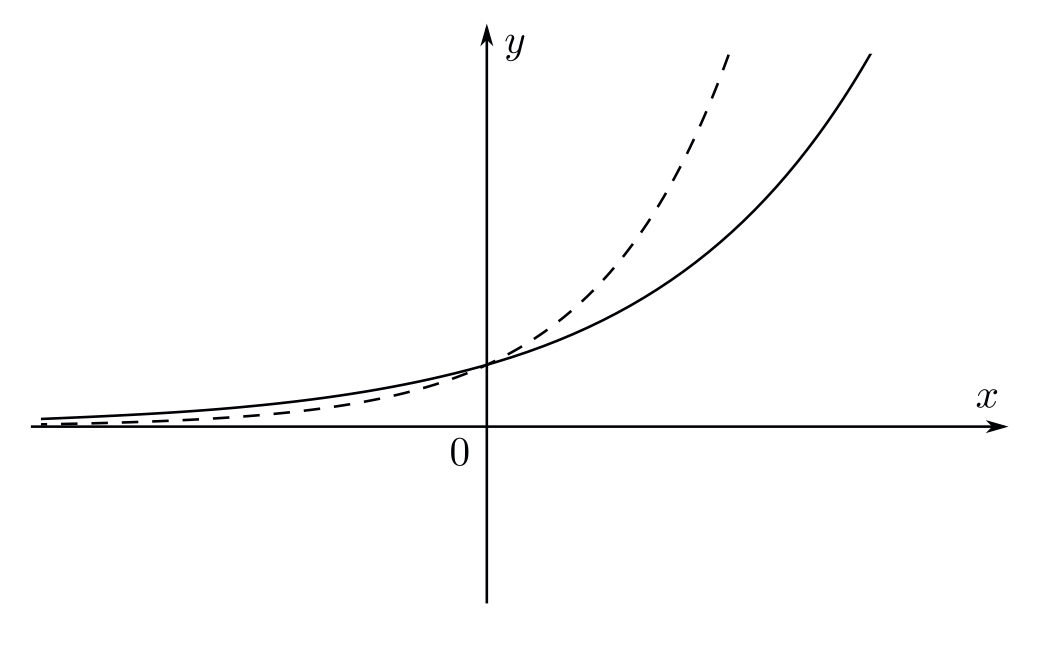
\includegraphics[width=0.6\linewidth]{tmua-2017-p2-q7.png}
    \caption{TMUA 2017 P2 Q7}
    \label{fig:tmua-2017-p2-q7}%
\end{figure}

\begin{example}[TMUA 2016 P2 Q17]
    Consider these simultaneous equations, where \(c\) is a constant:
    \begin{align*}
        y &= 3 \sin x + 2 \\
        y &= x + c
    \end{align*}

    Which of the following statements is/are true?

    \begin{enumerate}[label=\Roman*.]
        \item For some value of \(c\): there is exactly one solution with \(0 \leq x \leq \pi\) \textbf{and} there is at least one solution with \(-\pi < x < 0\).
        \item For some value of \(c\): there is exactly one solution with \(0 \leq x \leq \pi\) \textbf{and} there are no solutions with \(-\pi < x < 0\).
        \item For some value of \(c\): there is exactly one solution with \(0 \leq x \leq \pi\) \textbf{and} there are no solutions with \(x > \pi\).
    \end{enumerate}
\end{example}

To negate quantifiers, we have:
\begin{itemize}
    \item \(\lnot \pqty{\forall x: P\pqty{x}} = \exists x: \lnot P\pqty{x}\);
    \item \(\lnot \pqty{\exists x: P\pqty{x}} = \forall x: \lnot P\pqty{x}\).
\end{itemize}

In other words, we flip quantifiers and negate the following statement.

\subsection{Negating Statements}

We learnt above how to negate individual statements. Negating very long, combined statements is just repeated application of the previous separate parts.

\begin{example}
    Negating the statement ``for all \(n \in \ZZ\), \(n^2\) is even implies \(n\) is even'' gives ``there exists \(n \in \ZZ\) such that \(n^2\) is even and \(n\) is odd''.

    Negating the statement ``for all \(x\), there exists \(y\) such that \(y > x\)'' gives ``there exists \(x\) such that for all \(y\), \(y \leq x\)''.
\end{example}

\begin{example}[Numbers and Sets, Example Sheet 1 (2025), Q5 (i)]
    Let \(a, b, m, n \in \NN\). Negate the statement
    \[
        \forall m \exists n \forall a \forall b: \pqty{n \geq m} \land \bqty{\pqty{a = 1} \lor \pqty{b = 1} \lor \pqty{ab \neq n}}
    \]
\end{example}

\begin{problem}
    What is this statement saying?
\end{problem}

\begin{example}[Numbers and Sets, Example Sheet 1 (2025), Q5 (ii)]
    Negate the statement: if Bumrah is not a faster bowler than Tait, then Australia is worse than England in cricket.
\end{example}

\begin{example}[TMUA 2017 P2 Q17]
    A set \(S\) of whole numbers is called \emph{stapled} \textbf{if and only if} for every whole number \(a\) which is in \(S\) there exists a prime factor of \(a\) which divides at least one other number in \(S\).

    Let \(T\) be a set of whole numbers. Which of the following is true \textbf{if and only if} \(T\) is \textbf{not} stapled?

    \begin{enumerate}[label=\Alph*.]
        \item For every number \(a\) which is in \(T\), there is no prime factor of \(a\) which divides every other number in \(T\).
        \item For every number \(a\) which is in \(T\), there is no prime factor of \(a\) which divides at least one other number in \(T\).
        \item For every number \(a\) which is in \(T\), there is a prime factor of \(a\) which does not divide any other number in \(T\).
        \item For every number \(a\) which is in \(T\), there is a prime factor of \(a\) which does not divide at least one other number in \(T\).
        \item There exists a number \(a\) which is in \(T\), there is no prime factor of \(a\) which divides every other number in \(T\).
        \item There exists a number \(a\) which is in \(T\), there is no prime factor of \(a\) which divides at least one other number in \(T\).
        \item There exists a number \(a\) which is in \(T\), there is a prime factor of \(a\) which does not divide any other number in \(T\).
        \item There exists a number \(a\) which is in \(T\), there is a prime factor of \(a\) which does not divide at least one other number in \(T\).
    \end{enumerate}
\end{example}

\section{Proofs}
\subsection{Direct Deduction}

\textbf{Proof by direct deduction} for a statement is by starting from its hypotheses and making logical steps to reach the conclusion. For example, if we want to prove \(A \implies B\), then we can make the steps \(A \implies P\), \(P \implies Q\), \(Q \implies R\), \(R \implies B\) and combine them into
\[
    A \implies P \implies Q \implies R \implies B
\]
giving the proof.

\begin{example}[TMUA 2016 P2 Q7]
    The four real numbers \(a\), \(b\), \(c\) and \(d\) are all greater than \(1\). Suppose that they satisfy the equation
    \[
        \log_c d = \pqty{\log_a b}^2.
    \]

    Use some of the lines given to construct a proof that, in this case, it follows that
    \[
        \log_b d = \pqty{\log_a b} \pqty{\log_a c}.
    \]

    \begin{enumerate}
        \item Let \(x = \log_a b\) and \(y = \log_a c\) \vspace{1em}
        \item \(d = \pqty{c x}^2\)
        \item \(d = c^{\pqty{x^2}}\)
        \item \(d = b^{xy}\) \vspace{1em}
        \item \(d = \pqty{a^y}^{\pqty{x^2}}\)
        \item \(d = \pqty{\pqty{a^y}^x}^2\)
        \item \(d = \pqty{a^x}^{xy}\) \vspace{1em}
        \item \(d = a^{\pqty{y^{2x}}}\)
        \item \(d = a^{\pqty{x^2 y}}\)
    \end{enumerate}
\end{example}

\subsection{Contradiction}

\textbf{Proof by contradiction} of a statement of a form \(A \implies B\) is done by assuming \(\lnot B\), and using logical deduction to reach a result that contradicts with \(A\), i.e., we prove \(\lnot \pqty{A \land \pqty{\lnot B}}\) This is precisely proving the negation of the implication cannot be true.

Concretely speaking, to prove some statement \(A\), we:
\begin{itemize}
    \item start by assuming not \(A\) is true;
    \item logical deducting to two contradicting statements, \(B\) and \(\lnot B\);
    \item therefore our assumption not \(A\) is true must therefore be false;
    \item finally concluding that \(A\) must be true.
\end{itemize}

\begin{example}
    Prove that \(\sqrt{2}\) is irrational.
\end{example}

\subsection{Contraposition}

Recall a statement \(A \implies B\) is logically equivalent to \(\pqty{\lnot B} \implies \pqty{\lnot A}\). \textbf{Proof by contraposition} proves a statement of the form \(A \implies B\) by proving its contrapositive, an equivalent statement.

\subsection{Casework}

\textbf{Proof by cases} is by considering all possible cases that a variable in the assumption can take, and show that they all lead to the result we want to prove.

\begin{example}
    Let \(x \in \ZZ\). Prove that \(x^2\) has a remainder of \(0\) or \(1\) upon division by \(3\).
\end{example}

\subsection{Counterexample}

To disprove a statement of the form
\[
    \forall x \in S: A\pqty{x} \implies B\pqty{x},
\]
we may find some \(x \in S\), such that \(A\pqty{x}\) is \textbf{true} but \(B\pqty{x}\) is \textbf{false}. This is called a \textbf{counterexample}.

\begin{example}[TMUA 2016 P2 Q5]
    Consider the statement: a number \(n\) is prime if it is \(1\) less or \(5\) less than a multiple of \(6\).

    How many counterexample are there in the range \(0 < n < 50\)?
\end{example}

\begin{example}[TMUA 2017 P2 Q5]
    Consider the following three statements:
    \begin{enumerate}[label=\Roman*.]
        \item \(10 p^2 + 1\) and \(10 p^2 - 1\) are both prime when \(p\) is an odd prime.
        \item Every prime greater than \(5\) is of the form \(6n + 1\) for some integer \(n\).
        \item No multiple of \(7\) greater than \(7\) is prime.
    \end{enumerate}

    The result \(91 = 7 \times 13\) can be used to provide a counterexample to which of the above statements?
\end{example}

\subsection{Common Errors}

TMUA asks us to identify errors in a proof given. The following is a list of common errors that appear in those.

\paragraph{Square roots and squaring equations.} Squaring equations gives extra solutions: this means \(x = y^2\) does not imply \(\sqrt{x} = y\).

\begin{example}
    To solve the equation \(x + 1 = 4\), we square both sides to get \(x^2 + 2x + 1 = 16\), which reduces to \(\pqty{x + 5} \pqty{x - 3} = 0\). Hence, \(x = -5\) or \(x = 3\).

    The solution \(x = -5\) is introduced because of squaring the original equation.
\end{example}

\paragraph{Incorrectly dealing with inequality signs.} For example, one may incorrectly assume \(x < y\) implies \(x^2 < y^2\), or \(a < b\) implies \(ac < bc\) (which are both not true).

\paragraph{Incorrectly dealing with functions.} For example, one may incorrectly assume \(x < y\) implies \(f\pqty{x} < f\pqty{y}\) for some non-trivial function, say \(f\pqty{x} = \pqty{\flatfrac{1}{2}}^x\). Or the converse: one may incorrectly assume that \(\abs{x} = \abs{y}\) implies \(x = y\).

\paragraph{Dividing by zero.} One may incorrectly assume that \(ac = bc\) necessarily implies \(a = b\).

\begin{example}
    Identify the error in the following proof.

    \begin{itemize}
        \item Let \(x\) and \(y\) be non-zero numbers such that \(x = y\).
        \item The nwe can write \(x^2 = xy\).
        \item Subtracting \(y^2\) from both sides gives \(x^2 - y^2 = xy - y^2\).
        \item Factorising gives \(\pqty{x + y} \pqty{x - y} = y \pqty{x - y}\).
        \item Therefore, dividing by \(\pqty{x - y}\) gives \(x + y = y\).
        \item As \(x = y\), we have \(2y = y\).
        \item Dividing by the non-zero \(y\), we have \(2 = 1\).
        \item Subtracting \(1\) from both sides, we have \(1 = 0\).
    \end{itemize}
\end{example}

\begin{example}[TMUA 2016 P2 Q13]
    In this question, \(a\), \(b\), and \(c\) are positive integers.

    The following is an attempted proof of the false statement: If \(a\) divides \(bc\), then \(a\) divides \(b\) or \(a\) divides \(c\). [\(a\) divides \(bc\) means \(a\) is a factor of \(bc\)]

    Which line contains the error in this proof?

    \begin{enumerate}
        \item The statement is equivalent to `if \(a\) does not divide \(b\) and \(a\) does not divide \(c\) then \(a\) does not divide \(bc\)'.
        \item Suppose \(a\) does not divide \(b\) and \(a\) does not divide \(c\). Then the remainder when dividing \(b\) by \(a\) is \(r\), where \(0 < r < a\), and the remainder when dividing \(c\) by \(a\) is \(s\), where \(0 < s < a\).
        \item So \(s = ax + r\) and \(c = ay + s\) for some integers \(x\) and \(y\).
        \item Thus \(bc = a \pqty{axy + xs + yr} + rs\).
        \item So the remainder when dividing \(bc\) by \(a\) is \(rs\).
        \item Since \(r > 0\) and \(s > 0\), it follows that \(rs > 0\).
        \item Hence \(a\) does not divide \(bc\).
    \end{enumerate}
\end{example}

\begin{example}[TMUA 2017 P2 Q9]
    Consider the following attempt to prove this true theorem:

    \textbf{Theorem.} \(a^3 + b^3 = c^3\) has no solutions with \(a\), \(b\) and \(c\) positive integers.

    \textit{Attempted Proof}. Suppose that there are positive integers \(a\), \(b\) and \(c\) such that \(a^3 + b^3 = c^3\).

    \begin{enumerate}[label=\Roman*.]
        \item We have \(a^3 = c^3 - b^3\).
        \item Hence \(a^3 = \pqty{c - b}\pqty{c^2 + cb + b^2}\).
        \item It follows that \(a = c - b\) and \(a^2 = c^2 + cb + b^2\), since \(a \leq a^2\) and \(c - b \leq c^2 + cb + b^2\).
        \item Eliminating \(a\), we have \(\pqty{c - b}^2 = c^2 + cb + b^2\).
        \item Multiplying out, we have \(c^2 - 2cb + b^2 = c^2 + cb + b^2\).
        \item Hence \(3cb = 0\) so one of \(b\) and \(c\) is zero.
    \end{enumerate}

    But this is a contradiction to the original assumption that all of \(a\), \(b\) and \(c\) are positive. It follows that the equation has no solutions.

    Comment on this proof by choosing one of the following options:
        
\begin{enumerate}[label=\Alph*.]
    \item The proof is correct
    \item The proof is incorrect and the first mistake occurs on line I
    \item The proof is incorrect and the first mistake occurs on line II
    \item The proof is incorrect and the first mistake occurs on line III
    \item The proof is incorrect and the first mistake occurs on line IV
    \item The proof is incorrect and the first mistake occurs on line V
    \item The proof is incorrect and the first mistake occurs on line VI
\end{enumerate}
\end{example}

\begin{example}[TMUA 2017 P2 Q18]
    Consider the following problem: solve the inequality
    \[
        \pqty{\frac{1}{4}}^n < \pqty{\frac{1}{32}}^{10},
    \]
    where \(n\) is a positive integer.

    A student produces the following argument:
    \begin{align*}
        \pqty{\frac{1}{4}}^n &< \pqty{\frac{1}{32}}^{10} \\
        &\Downarrow && \text{(I)} \\
        \log_{\frac{1}{2}} \pqty{\frac{1}{4}}^n &< \log_{\frac{1}{2}} \pqty{\frac{1}{32}}^{10} \\
        &\Downarrow && \text{(II)} \\
        n \log_{\frac{1}{2}} \pqty{\frac{1}{4}} &< 10 \log_{\frac{1}{2}} \pqty{\frac{1}{32}} \\
        &\Downarrow && \text{(III)} \\
        n &< \frac{10 \log_{\frac{1}{2}} \pqty{\frac{1}{32}}}{\log_{\frac{1}{2}} \pqty{\frac{1}{4}}} \\
        &\Downarrow && \text{(IV)} \\
        n &< \frac{10 \times 5}{2} = 25 \\
        &\Downarrow && \text{(V)} \\
        1 &\leq n \leq 24
    \end{align*}

    Which step (if any) in the argument is invalid?

    \begin{enumerate}[label=\Alph*.]
        \item There are no invalid steps; the argument is correct
        \item Only step (I) is invalid; the rest are correct
        \item Only step (II) is invalid; the rest are correct
        \item Only step (III) is invalid; the rest are correct
        \item Only step (IV) is invalid; the rest are correct
        \item Only step (V) is invalid; the rest are correct
    \end{enumerate}
\end{example}

\end{document}